\documentclass[titlepage, 12pt, leqno]{article} % -------------------------------------------------- %
% -------------------- PACKAGES -------------------- %
% -------------------------------------------------- %
\usepackage{import}
\usepackage{hyperref}
\usepackage{setspace}
\usepackage{pdfpages}
\usepackage{mathtools}
\usepackage{transparent}
\usepackage{enumitem}
\usepackage{xcolor}
\usepackage{tcolorbox}
\usepackage{amsmath}
\usepackage{amssymb}
\usepackage{parskip}
\usepackage{graphicx}
\usepackage{bbm}
\usepackage[margin = 1in]{geometry}
\tcbuselibrary{breakable}
\tcbset{breakable = true}
\hfuzz=1pt


% -------------------------------------------------- %
% -------------- CUSTOM ENVIRONMENTS --------------- %
% -------------------------------------------------- %
\newtcolorbox{note}{colback=black!5!white,
                          colframe=black!55!white,
                          fonttitle=\bfseries,title=Note}

\newtcolorbox{ex}{colback=blue!5!white,
                          colframe=blue!55!white,
                          fonttitle=\bfseries,title=Example}

\newtcolorbox{definition}{colback=red!5!white,
                          colframe=red!55!white,
                          fonttitle=\bfseries,title=Definition}


% -------------------------------------------------- %
% ------------------- COMMANDS --------------------- %
% -------------------------------------------------- %
% Brackets, braces, etc. 
\newcommand{\abs}[1]{\lvert #1 \rvert}
\newcommand{\bigabs}[1]{\Bigl \lvert #1 \Bigr \rvert}
\newcommand{\bigbracket}[1]{\Bigl [ #1 \Bigr ]}
\newcommand{\bigparen}[1]{\Bigl ( #1 \Bigr )}
\newcommand{\ceil}[1]{\lceil #1 \rceil}
\newcommand{\floor}[1]{\lfloor #1 \rfloor}
\newcommand{\norm}[1]{\| #1 \|}
\newcommand{\bignorm}[1]{\Bigl \| #1 \Bigr \| #1}
\newcommand{\inner}[1]{\langle #1 \rangle}
\newcommand{\set}[1]{{ #1 }}


% -------------------------------------------------- %
% -------------------- SETUP ----------------------- %
% -------------------------------------------------- %
\title{\Huge{Voter Turnout as a Silver Lining to Political Polarization}}
\author{\large{Mitch Harrison, Cameron Martinez-Piedra, Tino Lopez}}
\date{\today}   
\begin{document}
\setlength{\parskip}{1\baselineskip}
\setlength{\parindent}{15pt}
\maketitle
\tableofcontents
\doublespacing
\newpage


% -------------------------------------------------- %
% --------------------- BODY ----------------------- %
% -------------------------------------------------- %
\section{Abstract}

Political polarization is rising in the United States and other OCED nations 
[1]. Most politically engaged citizens have some grasp on the negative
implications of such political shifts: damaging rhetoric, undemocratic 
sentiment, public distrust, and others. However, we seek to find a potential
silver lining: an increase in polarization could mean an increase in political
engagement and, thereby, voter turnout. We construct an approximate simulation
of the US electorate, modeling changes in mood over time. Every four years, we
tabulate an election and count the results. The results are grim: while 
partisans are much more likely to turn out to the polls, their fervor does not
translate to a larger population-level turnout.

\section{Introduction}
Democracy, as a political system, is the cornerstone of the United States of
America. It has encouraged citizen engagement by giving the people a voice in
shaping the nation's policies and directions. The most prominent example of
citizens' power is their collective ability to elect the President of the 
United States. However, several citizens refrain from using the power that
democracy grants them by not voting in presidential elections. Voter turnout 
is a fundamental pillar of any thriving democracy, serving as a vital gauge of
civic engagement and an instrument through which citizens assert their 
collective will. When a significant portion of the eligible population
participates in elections, the results are legitimized, reducing the risk of a
minority political party gaining disproportionate power. 

Encouraging higher voter turnout fosters a culture of civic engagement and
political participation, which may result in a more politically active
electorate. Effective democracy demands robust civic engagement, a significant
aspect of which is aggregate voter turnout. Nevertheless, despite the
importance of voting to sustain a democratic system, many fail to turn out.
The 2020 presidential election had the highest voter turnout since 1960, with
66\% of eligible voters turning out [11]. That is, in its best year,
approximately a third of the population of the United States failed to turn
out. This apparent political indifference drove us to research potential causal
factors in voter turnout, specifically the influence of observed increases in
political polarization [1].

The United States has continued to observe increasing political polarization 
[1]. This extreme polarization has several adverse effects, often leading to
extreme rhetoric and partisanship and fostering an environment of hostility and
demonization of the opposition. However, despite political polarization's
predominantly negative implications, we posit a potential silver lining in an
increase in voter turnout. Current research on the potential positive effect on
voter turnout by political polarization in the last decade is limited. However,
researchers have observed increased turnout after polarization in Germany, 
Spain, and the Netherlands [6]. Although turnout was higher in 2020 than at any
time since 1960 (Figure 1) [13], it may not have been extreme enough to account
for the disproportionate increase in political polarization when compared to
other OCED nations [1].

\begin{figure}[ht]
    \centering
    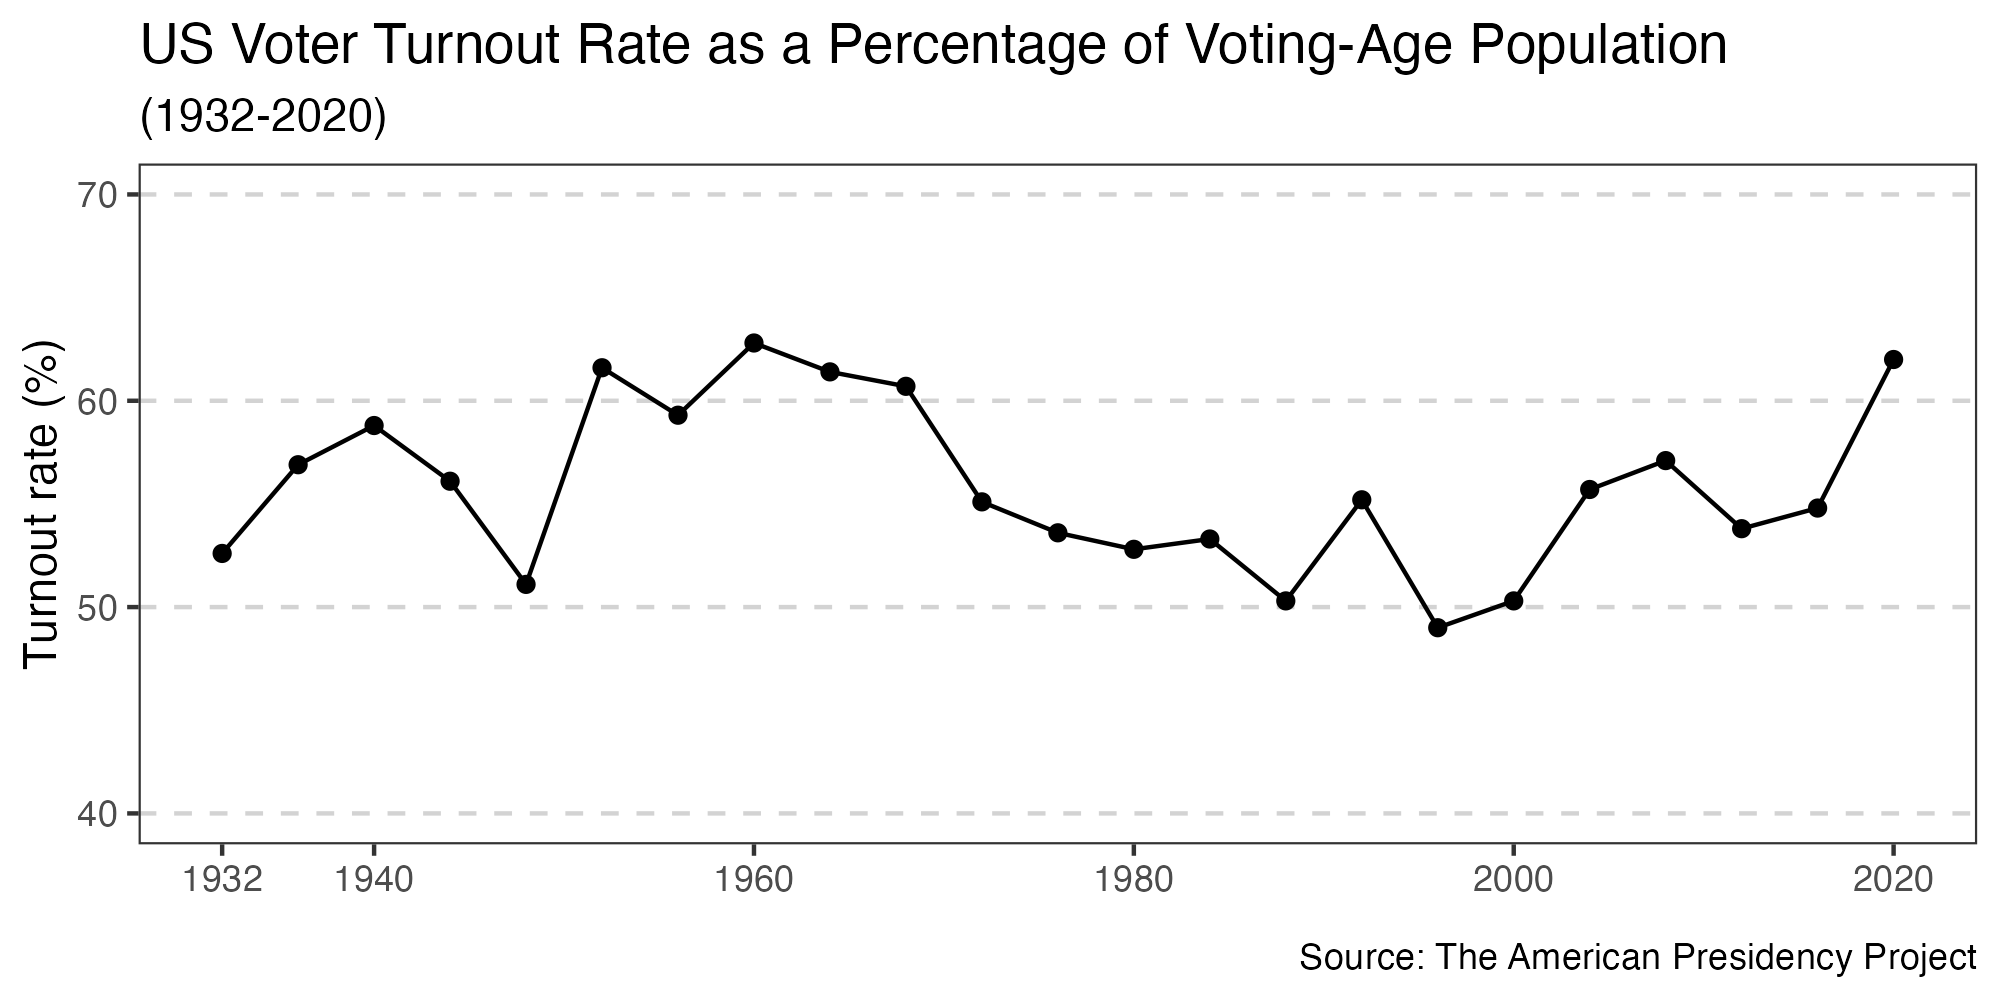
\includegraphics[width = 0.8\textwidth]{../plots/us_turnout.png}
    \caption{Total US voter turnout}
    \label{fig:label}
\end{figure}

\pagebreak
\section{Literature Review}
This study aims to explore the correlations and relationships between voter
turnout and various independent variables. Using demographic data alongside
information from past elections, we quantify the importance of one's vote, age,
political polarization, partisanship, and gender to their turnout likelihood.
These data are crucial to assembling our model and understanding how each
variable changes voter turnout. To accomplish this, we relied on external
sources, including data from the Pew Research Center, to facilitate our
investigation of these relationships.

In the initial phase of our research, we sought to better understand
voter turnout in past elections by utilizing the resources offered by 
the Pew Research Center. Notably, the 2018, 2020, and 2022 elections
recorded the highest voter turnouts in recent United States history 
[10]. Historical evidence shows that past elections can help understand why
people turn out to vote. We observed that voter participation is more likely 
when political outcomes are uncertain due to closely divided politics, as
individuals believe their votes can impact the results. The data provided by 
the Pew Research Center demonstrated that the proportion of major American
political parties is relatively even. That is, a comparatively small number of
votes can swing an election to either party [8]. Conversely, lower voter
participation occurred when people perceived their preferred political choice 
had minimal chance of winning. Individuals who believed their votes could 
effect change were more likely to turn out to vote. Those who thought their vote
held little significance were less likely to participate. Hence, it is essential
to recognize that higher voter turnout is associated with competitive political
landscapes and the belief that votes can make a difference. Additionally, other
factors, such as age, played a role in determining voter turnout.

The Pew Research Center's data enabled us to explore how age influences
political affiliations and typologies. Our study benefited from this 
information, which revealed that younger demographics tend to lean more liberal
while older demographics lean more conservative [2]. This data, derived from a
survey of over 10,000 Americans, identified four age groups (18-29, 30-49, 
50-64, and 65+) and assessed the strength of individuals' political preferences.
It was evident that the younger demographic (18-29) was inclined to be strongly
liberal, with approximately 70\% expressing this preference, while the 65+ age
group had 41\% identifying as conservative [2]. This analysis showed a
substantial shift towards conservatism as age increased. However, it is 
essential to note that while there were some strong liberals or conservatives, a
significant portion remained less firmly affiliated with any political party.

The literature also shows that political views often form at a young age,
influenced by family generations. An individual's birth era can significantly
impact political preferences [9]. Consequently, political choices change once
individuals can make independent decisions without the influence of their 
family. As individuals reach the age categories of 30-49 and 50-64, they tend to
make more informed decisions based on their life experiences, leading to
significant shifts in voting patterns [2]. Once these changes occur, individuals
often maintain consistent voting preferences. Although this does not explain all
aspects of voting behavior, it provides valuable insights into why certain age
groups exhibit higher turnout rates.

Politics and voter turnout are highly affected by an individual's race
and ethnicity [9]. Race and ethnicity are frequently central to an individual's
political affiliation [9]. The Pew Research Center provided statistics that 
white Americans are the most likely to turn out. However, racial minorities are
not monolithic, with support for Democrats and Republicans varying widely among
different racial minority groups. Our model uses these varying beliefs to adjust
starting political scores for agents of each racial group.

Older adults experience less physical mobility, meaning they are less
likely to move frequently and thus do not need to re-register to vote. Moreover,
they have more free time after retirement, providing a strong incentive to vote,
particularly regarding issues related to social security and income. In 
contrast, younger voters are often actively employed or enrolled in school, 
which may hinder their ability to participate in elections. These phenomena
combine to result in much higher turnout among older adults (as shown by Our
World in Data [4]) than younger ones, which we quantify as agent parameters in
our model, updating turnout likelihood as a voter ages.

Political polarization is crucial to understanding why individuals hold strong
political beliefs and vote accordingly. Pew finds that voters on the far end of
both sides of the political spectrum are more likely to show up on election day
[8]. We adjust agent turnout likelihoods similarly, increasing turnout rate when
an agent holds strong partisan beliefs. Those with mixed or less passionate
affiliations are less likely to participate [8]. This polarization, combined 
with age-related factors, contributes to the complex landscape of political
preferences, resulting in a sizable portion of voters with mixed or changing
political ideologies. Those who felt that they were not represented well by
either party and were in the "mixed" category (i.e., those who do not have a
strong association with any party) had lower turnout rates. This engagement
disparity can be attributed to various factors, including education, age, and
especially the strength of partisan leanings.

Education can also affect who turns out. Education levels significantly 
influence voter turnout, as higher-educated individuals tend to lean more 
liberal and more likely to show up on polling day [7]. At each iteration, our
model adjusts for these partisan and engagement changes based on the education
status of an individual agent.

The Center For American Women and Politics provided critical data related to
gender and voter turnout [5]. Contrary to our initial assumptions, women have
consistently turned out to vote more than men since the 1980 presidential
election [5]. This trend is influenced by the political preferences of women,
who tend to lean more liberal than men [9]. Consequently, our simulation 
slightly shifts female agents to the political left while increasing their
turnout at each iteration.

\subsection{Limitations of existing research}
Despite the insights gained from our research, some crucial limitations are 
worth noting before exploring our model outcomes. First, we had to make
generalizations regarding the impact of various parameters on individuals, such
as education. Educational backgrounds vary widely, and not all degrees or levels
of education are equal. While we would have loved a linear regression model to
help select the numeric strength on partisan lean/turnout likelihood while other
parameters are held constant, no such model is publically available at the time
of writing this piece. Additionally, each education system and institution
differs, making generalizations necessary for our analysis that have much higher
variance in the real-world citizenry. We also faced challenges in understanding
the strength of political ideology in individuals, as each person may have a
different level of attachment to their beliefs. While efforts have been made to
quantify political lean numerically, an agreed-upon standard has yet to form. 

Moreover, our study did not consider the family history of our agents, which can
shift partisan leanings, especially among younger voters who are still 
culturally tied to their parents. Our model, therefore, considers each agent
independently of all others. 

Finally, survey-based research inherently relies on voluntary participation,
which may introduce bias, and therefore, the data cannot fully represent the
entire US population of registered voters. While demographers and statisticians
work hard to account for these biases, we must acknowledge that variance is 
added each time survey results are used to quantify model shifts numerically. 
\pagebreak

\section{Methodology}
To investigate the effect of political polarization on voter turnout, we built
a highly simplified model of the United States. We drew age, race, and 
education levels from probability distributions observed by demographers 
[1, 7, 8, 9]. We evolved this population over time, replacing citizens from a
draw of the same joint demographic distribution as elders died with a 
probability observed by the NIH [3]. At each iteration, our agents' politics
shifted according to approximate expectations observed in recent elections [7].
Every four iterations (i.e., every four years), an election is held and results
are tabulated.

We quantify agents' politics on a continuous scale in which increasing negative
values are increasingly liberal, and positive values are increasingly
conservative. Agent political "scores" are shifted based on the strength of
correlations between parameters and US voter politics. For example, because 
black Americans are highly likely to lean Democrat [10], race pushes agent
politics score more negative than for other races. 

After agent traits are shifted at each iteration, each affects voter turnout
probability. Specifically, we model agent turnout likelihood as a Gaussian
distribution with a variable mean. An agent votes when the value drawn from 
that Gaussian distribution exceeds 0.5. The mean of this Gaussian distribution
varies as a function of each agent parameter after shifting them. 

Elections are held every four years (i.e., every four model iterations). Ties 
are broken arbitrarily with a probability of 0.5 for each party. Centrists are
identified as agents using the following formula,
\[
A_{c} = 
\begin{cases}
    1 & |A_{p}| < 0.1 \\
    0 & \text{otherwise}
\end{cases}
\]
where $A_{c} \in \{0,1\}$ is the agent's centrism status and $A_{p}$ is that
agent's political score. 

Centrists have some specific qualities: as a party is in power longer, their
political scores drift in the opposite direction of the sitting leader
(representing the general trend of declining presidential approval rating with
time [12]), and centrists drift further conservative with age than 
non-centrists do, which helps correct with an observed general shift away from
centrism with age [7].

Similarly to centrists, we quantify a separate agent status for "extremism." 
An agent is classified as "extreme" using the following,
\[
A_{e} =
\begin{cases}
    1 & |A_{p}| > 0.3 \\
    0 & \text{otherwise}
\end{cases}
\]
where $A_{e} \in \{0,1\}$ is the agent's extremism status and $A_{p}$ is that
agent's political score. For both centrism and extremism, a value of 1 indicates
an affirmative status for those conditions.

Like centrists, extremists have some unique behavior. Specifically, extreme
agents have a slight bump to the expected value of their turnout distribution
draw in the form of a shift in the mean of the Gaussian distribution from whic
h turnout is drawn. This effect is similar to the impact on turnout likelihood
that being between the ages of 50 and 65 has. That is, the effect is by no 
means a guarantee that turnout will occur. Additionally, extremists' political
scores move further away from the party in power if that party is not their 
own and not at all if they are of the same party as the sitting leader.

What results from this model is a highly simplified approximation of the
American electorate with quantifiable polarization. This model allows us to
investigate whether or not political polarization can overcome the natural 
drifts in American public opinion. 

\section{Data Presentation}
We aim to find two outcomes of our model: first, an increase in political
polarization over time, and second, the effect of that polarization on total
voter turnout over time. First, we have to quantify our population's
polarization. Figure 2 shows that when compared to the starting distribution of
political scores initialized in our model, the mass of the political 
distribution shifted from being centered near 0 (i.e., politically centrist)
towards the wings of the distribution. This increase in variance demonstrates
increased political polarization over time, even as generations die and new
agents are introduced to the model. While left-leaning voters show more mass at
their end of the distribution, this is likely a product of a slightly left
-leaning starting distribution, the parameters of which we discuss in the
Methodology.

\begin{figure}[ht]
    \centering
    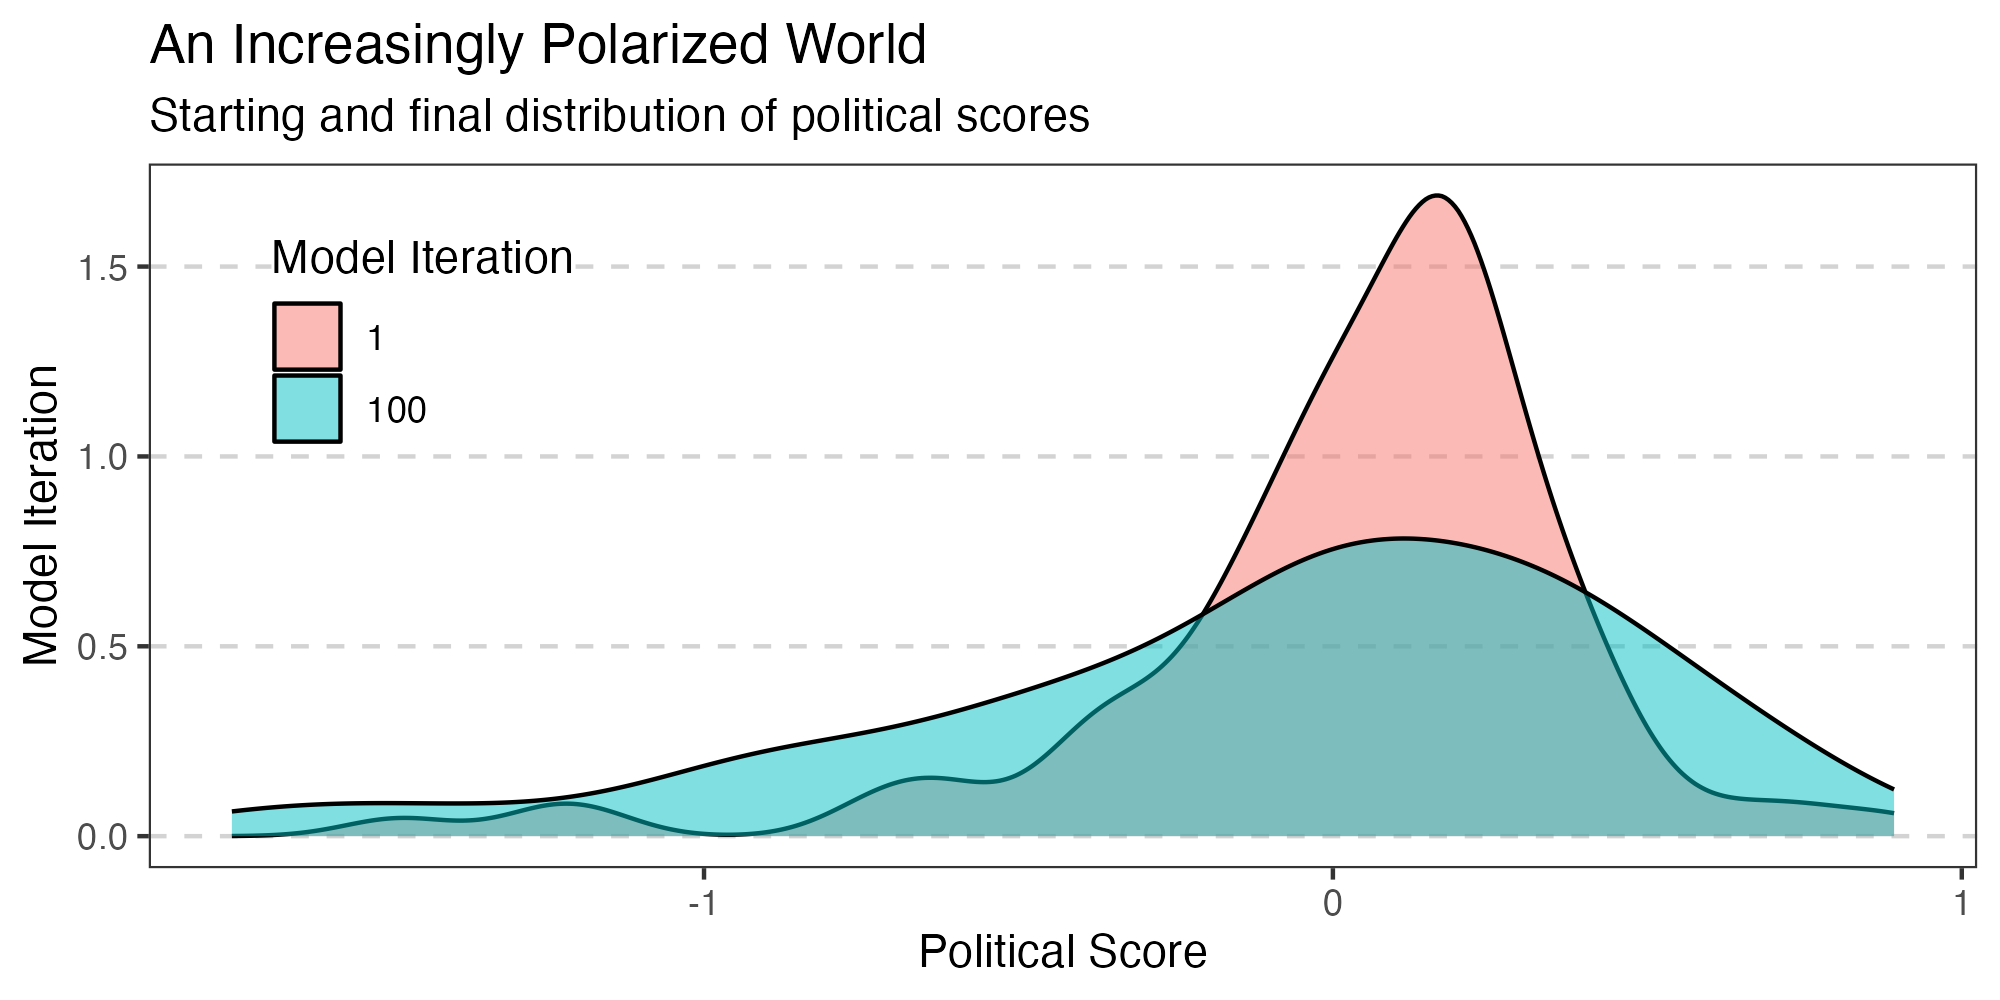
\includegraphics[width=0.8\textwidth]{../plots/polarization_change.png}
    \caption{Starting and final political score distribution}
\end{figure}

However, the story of our agents' polarization is more complex. While the
starting and ending distributions show a stark difference in politics, Figure 3
shows that comparative levels of polarization held once the initial 
polarization process took hold around iteration 40. This trend indicates that
in our model, while politics are a polarizing force, there is a threshold beyond
which a population, on average, is unwilling to cross en masse.

\begin{figure}[ht]
    \centering
    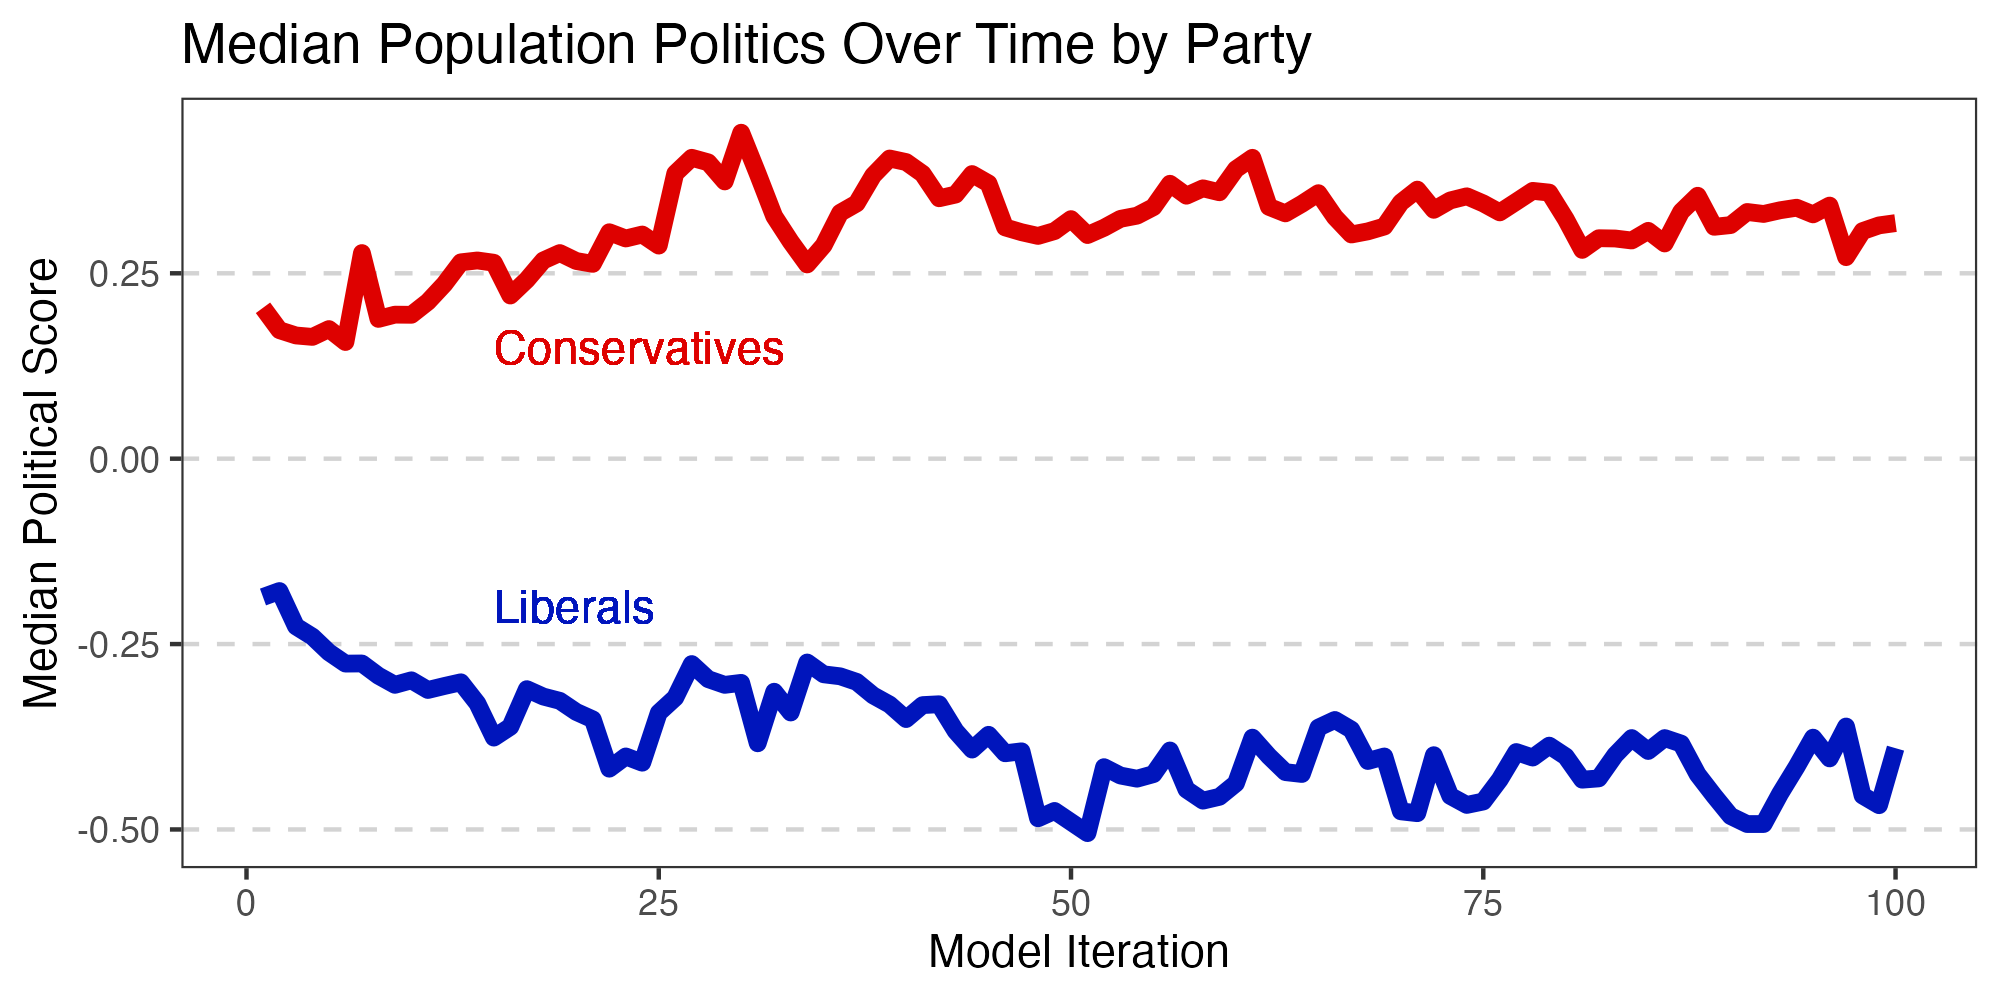
\includegraphics[width=0.8\textwidth]{../plots/median_pop_pol.png}
    \caption{Population political shifts by party}
\end{figure}
\pagebreak

Comparing the distribution of political scores among the population at 
iteration 40 and the final iteration shows a much closer trend. That is, once 
we allow a population to become polarized at approximately this rate, politics
stabilize and remain approximately identical until the model closes at iteration
100. We will call iteration 40 our "polarization equilibrium point." Figure 4 
shows population political distribution between our polarization equilibrium
and the final iteration of our model.

\begin{figure}[ht]
    \centering
    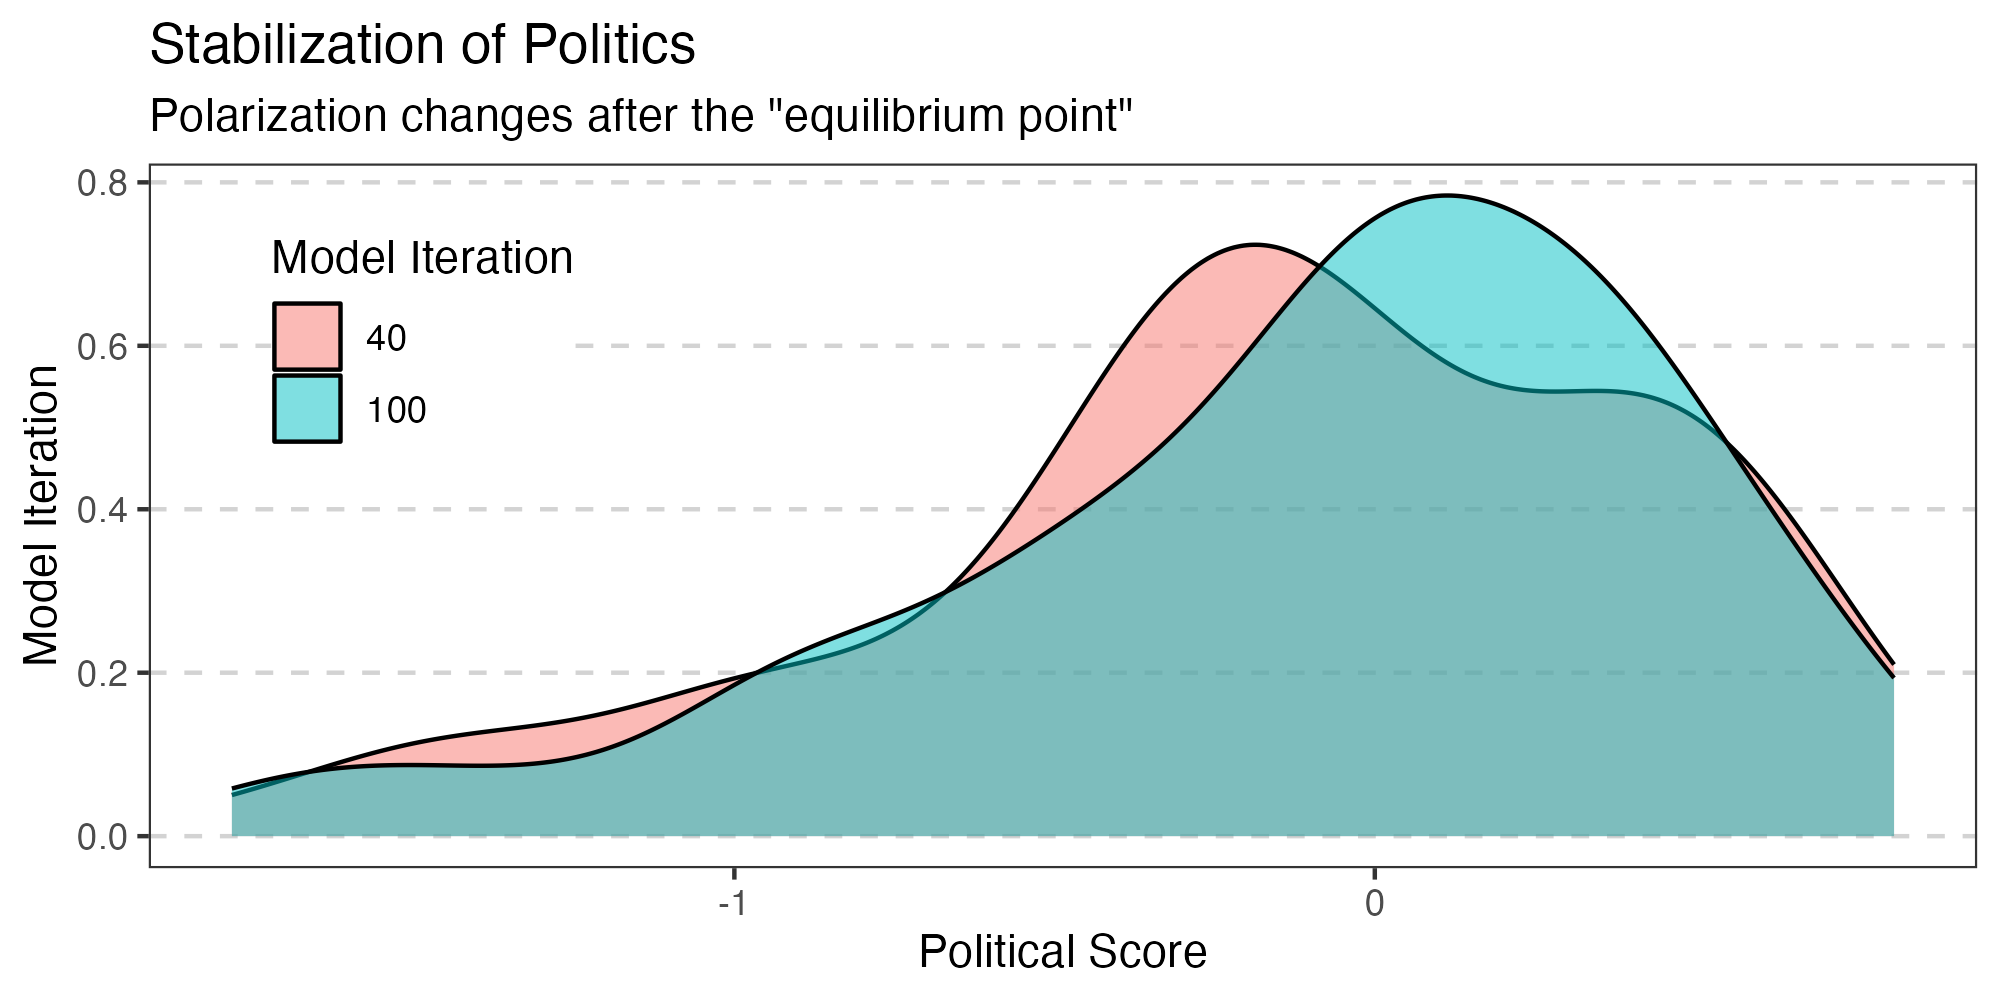
\includegraphics[width=0.8\textwidth]{../plots/polarization_40.png}
    \caption{Agent political shifts after iteration 40}
\end{figure}

Once polarization is quantified, we hope to find a relationship between that
polarization and an increase in voter turnout, on average, after polarization
occurs. Figure 5 shows the total votes cast (out of the 100-agent population) in
each election. After our polarization equilibrium at iteration 40, voting rates
remain approximately equivalent to the rates predating that equilibrium.
Additionally, while polarization was slightly stronger by liberal voters, 
exactly half of the post-equilibrium elections went to either party. In the
limited time since political polarization became a household phrase (i.e., since
the 2016 election cycle), one election has gone to each party, so these results
are unsurprising.

\begin{figure}[ht]
    \centering
    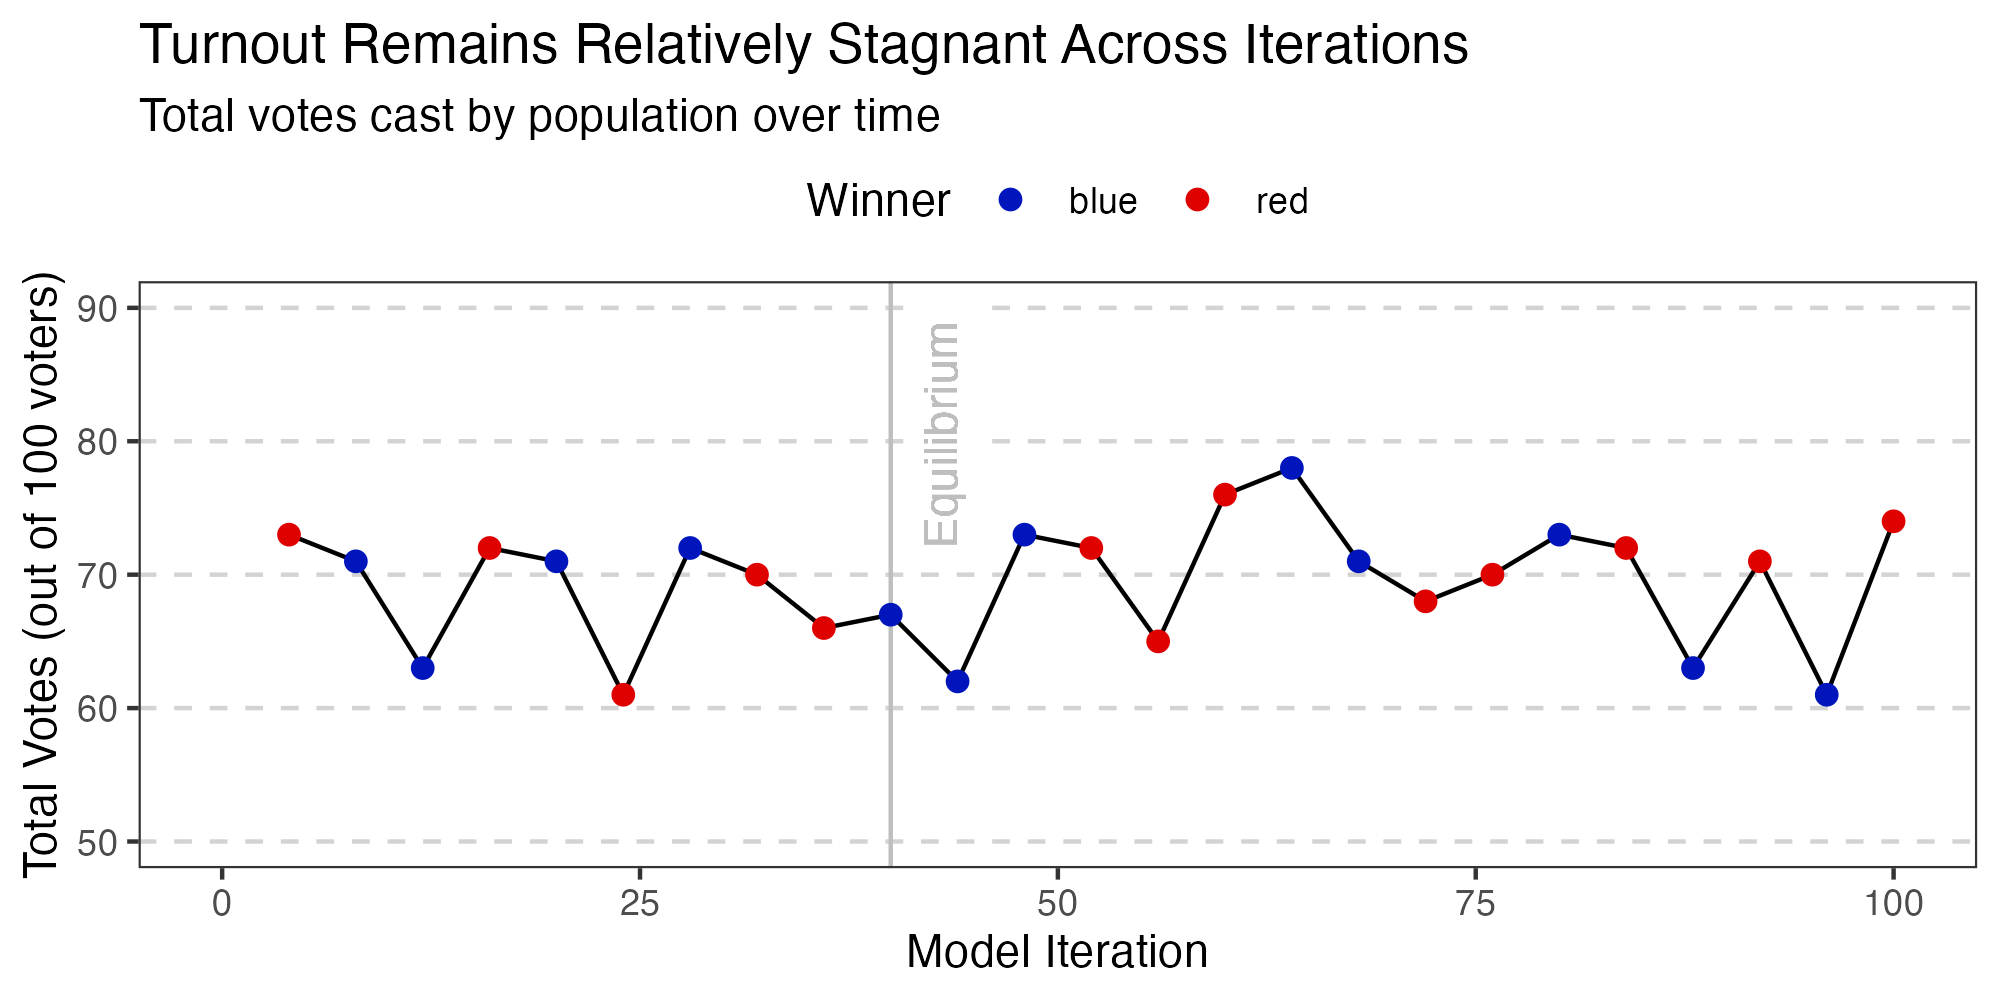
\includegraphics[width=0.8\textwidth]{../plots/total_votes.png}
    \caption{Total vote count over all electoral iterations}
\end{figure}

We find that, even as polarization takes hold, the absolute distribution of 
party loyalty remains remarkably similar. Our population's politics tend to
regress towards a mean of 0. That is, the natural push and pull of partisan
politics may make people more confident in their votes but does not necessarily
change the overall political party distribution of the population writ large.
Even as liberal voters became slightly more partisan conservatives, neither 
party took a firm majority over a long-run average. Figure 6 shows the
comparative number of agents in each party over every iteration of our model.
\pagebreak

\begin{figure}[ht]
    \centering
    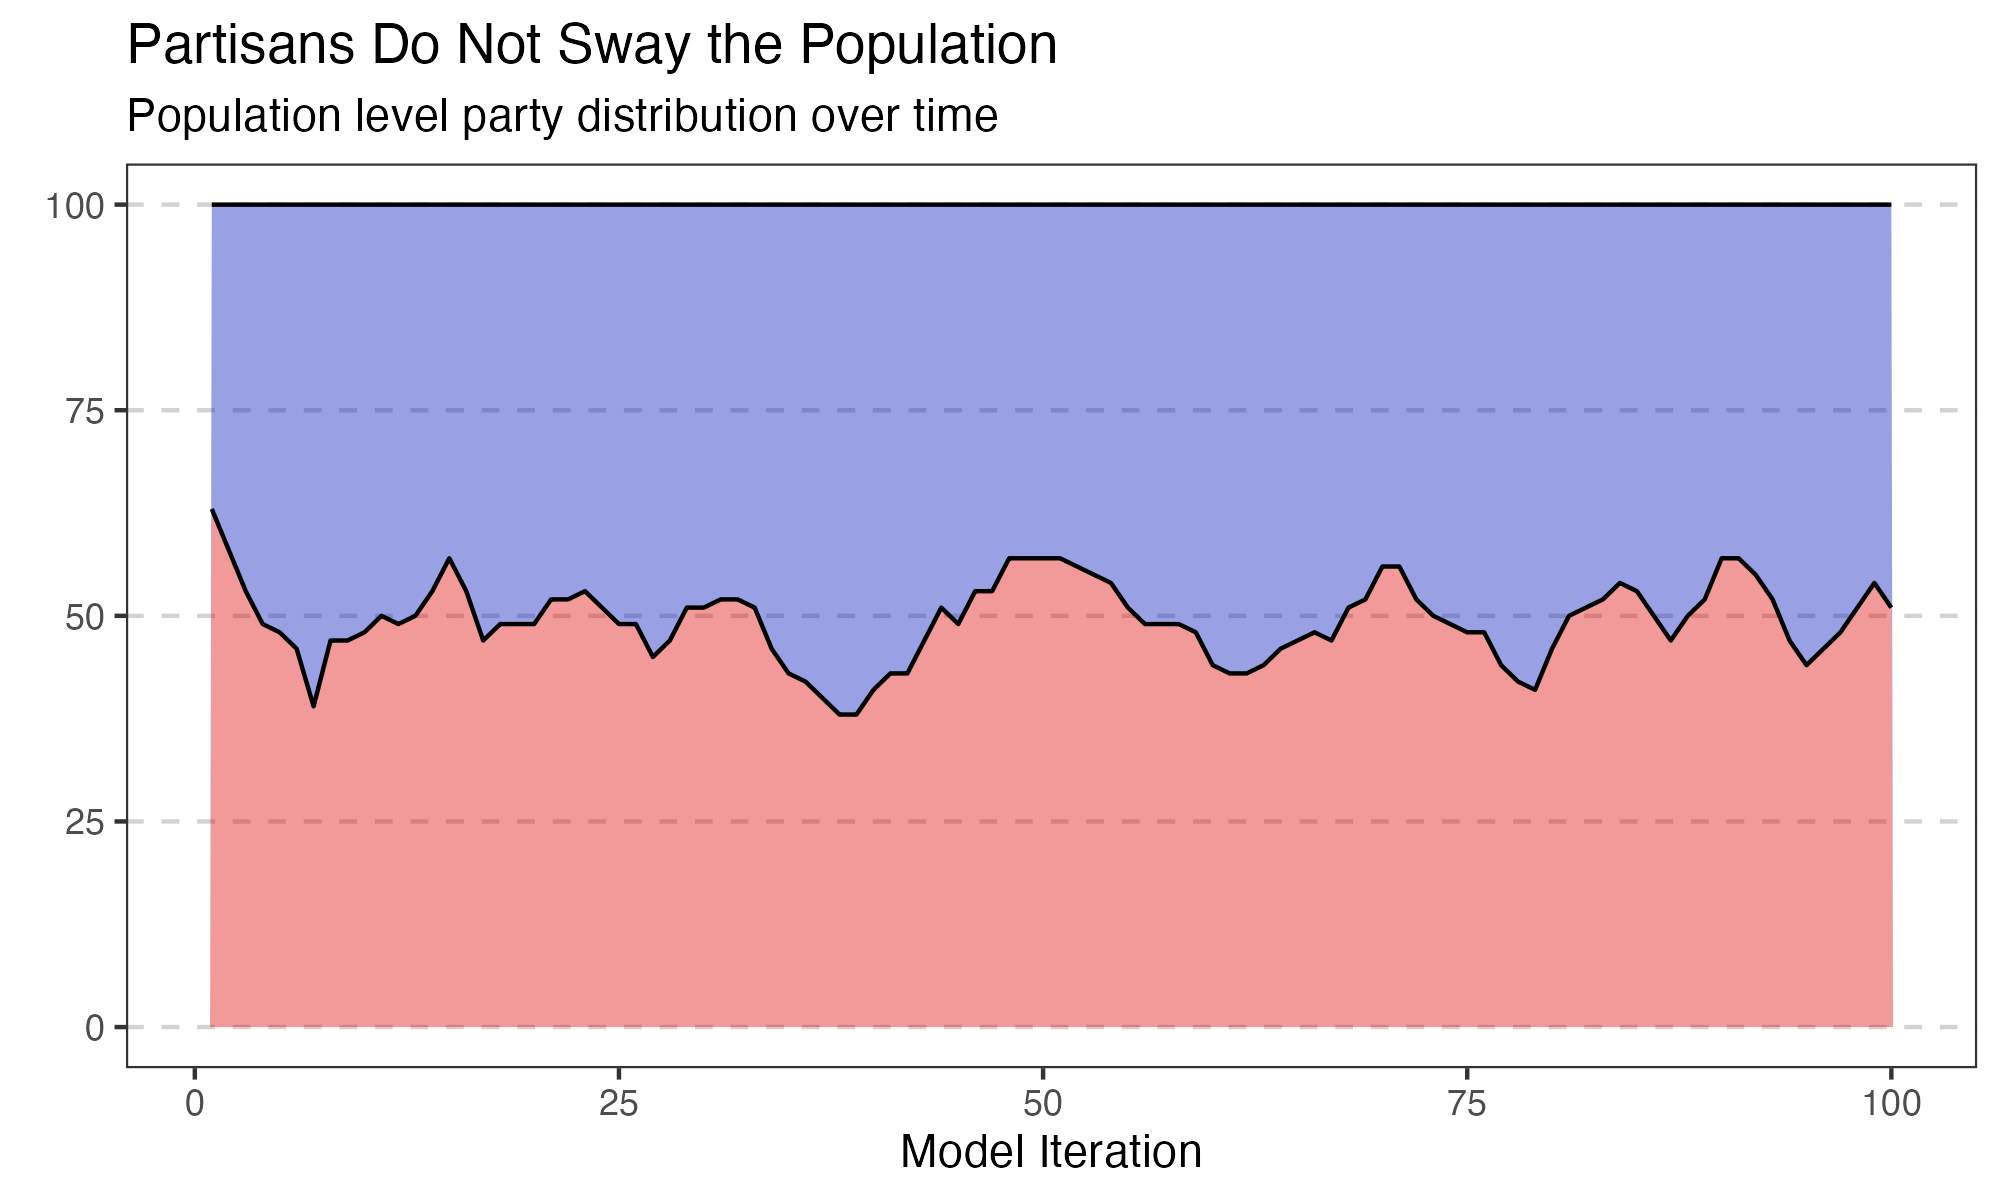
\includegraphics[width=0.8\textwidth]{../plots/party_dist.png}
    \caption{Population party distribution over all iterations}
\end{figure}

\section{Statistical Modelling}
We constructed a linear model using data from each simulated election year to
find which of our agent parameters had the most impact on whether or not a
voter turned out. It is important to note that this model is limited in its use
outside of this simulation since relationships between variables are sometimes
linear in our simulation, where they may not be in real-world practice. The
results of that model are shown in Table 1 below.

Unsurprisingly, an agent being an extremist is highly correlated with turnout.
This is expected behavior since increasing turnout likelihood with extremism was
built into our model. Similarly, an increase in age predicts an increase in
turnout likelihood. This is also built into our simulation, as it is an observed
phenomenon in real-world elections [2]. However, the findings of our linear 
model deviate from programmed simulation rules in two places. First, an agent is
more likely to vote if they are conservative. This was not explicitly added to
our model but is an observed phenomenon [7] that emerged naturally due to our
simulation parameters. Second, although education was explicitly coded to
increase turnout likelihood in our simulation, voting turnout rates did not vary
across education levels while holding all else constant. This is likely
attributable to an offsetting of the changes made to turnout likelihood by
education from a combination of other factors.

\begin{figure}[ht]
    \centering
    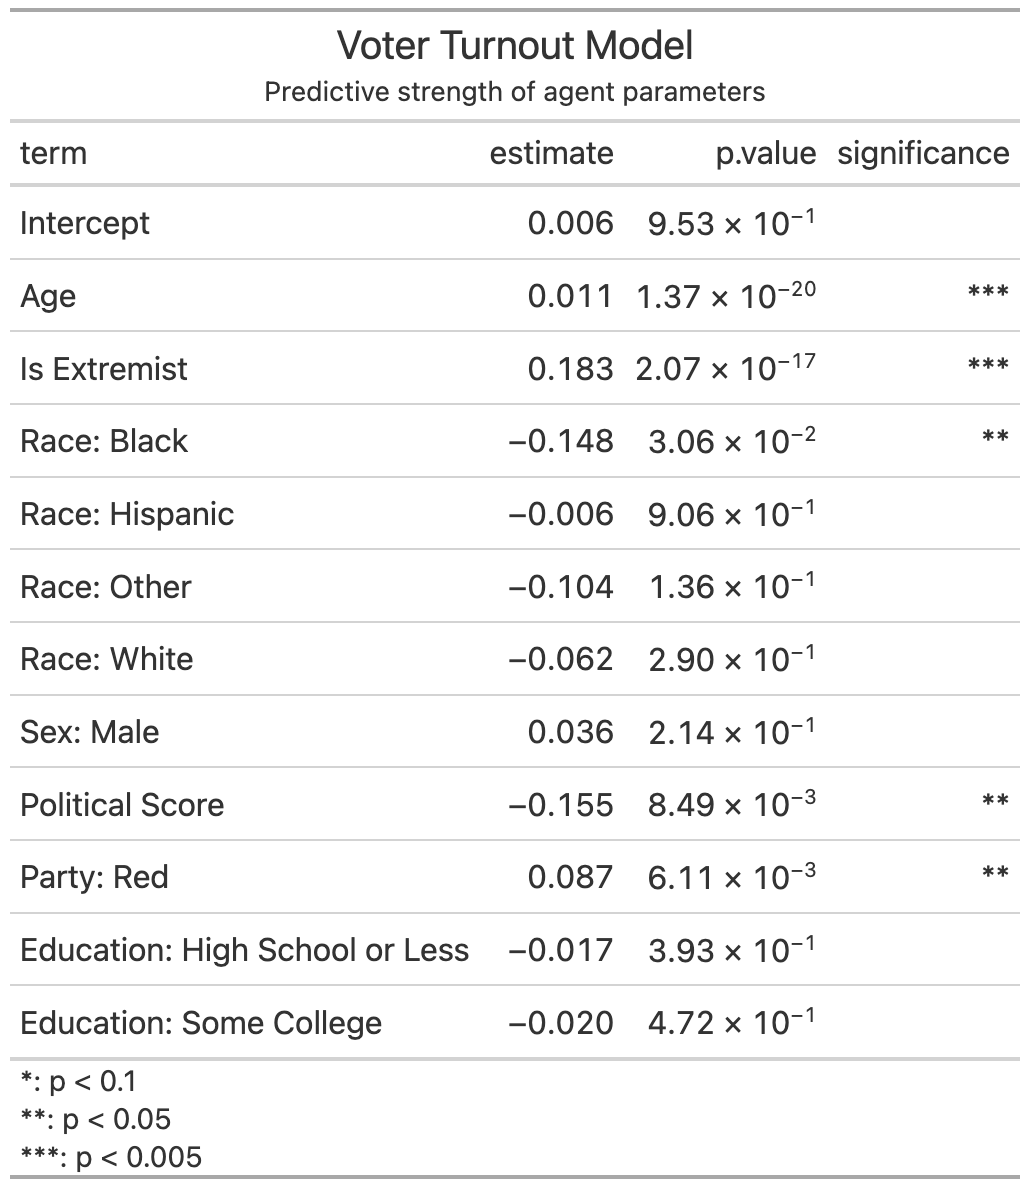
\includegraphics[width=0.6\textwidth]{../plots/table.png}
    \caption{Linear model output}
\end{figure}

Our linear model using simulated data shows that polarization is highly likely 
to increase the chances of any one agent turning out. However, on a population
level, our previous analysis shows no real change as political polarization
increases. Thus, while we did observe polarization, it did not have an
appreciable effect on long-term, population-level turnout levels.

\pagebreak
\section{Conclusion}
Despite the insights gained from our research, some crucial limitations are
worth noting before exploring our model outcomes. First, we had to make
generalizations regarding the impact of various parameters on individuals, such
as education. Educational backgrounds vary widely, and not all degrees or 
levels of education are equal. While we would have loved a linear regression
model to help select the numeric strength on partisan lean/turnout likelihood
while other parameters are held constant, no such model is publically available
at the time of writing this piece. Additionally, each education system and
institution differs, making generalizations necessary for our analysis that have
much higher variance in the real-world citizenry. We also faced challenges in
understanding the strength of political ideology in individuals, as each person
may have a different level of attachment to their beliefs. While efforts have
been made to quantify political lean numerically, an agreed-upon standard has 
yet to form. 

Moreover, our study did not consider the family history of our agents, which can
shift partisan leanings, especially among younger voters who are still 
culturally tied to their parents. Our model, therefore, considers each agent
independently of all others. 

Finally, survey-based research inherently relies on voluntary participation,
which may introduce bias, and therefore, the data cannot fully represent the
entire US population of registered voters. While demographers and statisticians
work hard to account for these biases, we must acknowledge that variance is
added each time survey results are used to quantify model shifts numerically. 

\subsection{Future Research}
There is much left to be done in the field of election outcome modeling. Most
importantly, demographers and survey writers must continue to improve their
numeric quantification of otherwise non-numeric phenomena. Additionally, forming
a widely accepted system of numeric quantification of partisan leanings would
allow researchers from all over the social sciences to use partisan lean in 
their work. In modeling specifically, social science would benefit significantly
from the creation of dedicated software (R library, Python package, or other) 
for agent-based election modeling. While building our own was an excellent
exercise in learning, saving time by using a robust and abstracted modeling
framework would have allowed us to focus more rigorously on our results.

\pagebreak
\section*{References}
\begin{enumerate}[label={[\arabic*]}]
    \item Boxell, L., Gentzkow, M., \& Shapiro, J. (2020). \textit{Cross-Country
        Trends in Affective Polarization.} https://doi.org/10.3386/w26669
    \item DeSilver, D. (2014, July 9). \textit{The politics of American 
        generations: How age affects attitudes and voting behavior.} Pew 
        Research Center. 
        https://www.pewresearch.org/short-reads/2014/07/09/the-politics-
        of-american-generations-how-age-affects-attitudes-and-voting-
        behavior/
    \item Edwards, R. D. (2008, June 1). \textit{The cost of uncertain life 
        span.} Journal of population economics. https://www.ncbi.nlm.nih.gov/
        pmc/articles/PMC3285408/
    \item \textit{Election voter turnout rate by age in the United States.} Our
        World in Data. (n.d.). https://ourworldindata.org/grapher/voter-turnout-
        rate-by-age-usa
    \item \textit{Gender differences in voter turnout.} Center for American 
        Women and Politics. (2023). https://cawp.rutgers.edu/facts/voters/gender
        -differences-voter-turnout
    \item Harteveld, E., \& Wagner, M. (2022). \textit{Does affective 
        polarisation increase turnout? Evidence from Germany, the
        Netherlands, and Spain.} West European Politics, 46(4), 732–759. 
        https://doi.org/10.1080/01402382.2022.2087395
    \item Newport, F. (2021, May 7). \textit{Party identification varies widely
        across the age spectrum.} Gallup.com. https://news.gallup.com/poll/
        172439/party-identification-varies-widely-across-age-spectrum.aspx
    \item Pew Research Center. (2016, April 26). \textit{A wider ideological gap 
        between more and less educated adults.} Pew Research Center - US 
        Politics \& Policy. 
        https://www. pewresearch.org/politics/2016/04/
        26/a-wider-ideological-gap-between-more-and-less-educated-adults/
    \item Pew Research Center. (2021, November 9). \textit{Political engagement 
        among typology groups.} Pew Research Center - US Politics \& Policy.
        https://www.pewresearch.org/ politics/2021/11/09/political-engagement-
        among-typology-groups
    \item Pew Research Center. (2018, March 20). \textit{Trends in party 
        affiliation among demographic groups.} Pew Research Center - US Politics 
        \& Policy. https://www.pewresearch.org/ politics/2018/03/20/1-
        trends-in-party-affiliation-among-demographic-groups/ 
    \item Pew Research Center. (2023, July 12). \textit{Voter Turnout, 2018-
        2022.} Pew Research Center. https://www.pewresearch.org/politics/2023/
        07/12/voter-turnout-2018-2022/
    \item Silver, N. (2023, November 11). \textit{How popular is Joe Biden?}
        FiveThirtyEight. https:// projects.fivethirtyeight.com/biden-approval-
        rating/?cid=rrpromo
    \item Elections | The American Presidency Project. (n.d.). https://www.
        presidency. ucsb.edu/statistics/data/voter-turnout-in-presidential-
        elections
\end{enumerate}

\end{document}
